\section{Retract: backflow and the membership gate}
\label{sec:retract}

The first three stages assume the store should keep what it has and get better at keeping it. Sometimes a fact must instead be made to leave --- a source is retracted, a user exercises a deletion right, a fact is confirmed wrong. This section asks whether ``deleting'' a fact from a compiled or agentic store actually makes it gone.

\subsection{Backflow: correctness-gated deletion does not stay deleted}

Consider an agent whose memory is not a flat store but a system that periodically \emph{consolidates}: it re-reads its own transcripts and evidence and re-derives and re-writes memory notes, the same rewrite-to-update pattern as \S\ref{sec:compile}--\S\ref{sec:maintain}. If a synthesized private fact $d$ is retracted --- its note deleted --- but the underlying observations that originally supported it are not also purged, we ask whether $d$ resurfaces on a later consolidation pass. We call this \textbf{backflow}.

We test two gate designs at the write-consolidate hook. A \textbf{correctness gate} (A2) admits any write that is faithful to the agent's surviving evidence, regardless of whether that write discloses the retracted fact --- this is the gate design an agent framework would use by default, since it is exactly what ``don't hallucinate, stay faithful to your memory'' asks for. A \textbf{membership veto} (A3) instead blocks any write matching a deletion-set membership predicate (canonicalized-value hash match, or embedding-cone similarity, or NLI entailment of the retracted fact), independent of whether the write is otherwise correct.

On $n{=}250$ synthetic private facts (per-arm $n{=}189$--$221$ after infrastructure-error filtering), the correctness gate leaves residual surfacing at $0.990$ --- statistically indistinguishable from no deletion at all (the no-gate baseline is $0.991$). The membership veto reaches $0.000$ ($95\%$ CI $[0, 0.019]$), matching a never-ingested oracle control. On the subset scored under both gates ($n{=}193$), the discrimination between them is $0.990$ (cluster-bootstrap $95\%$ CI $[0.974, 1.0]$, excluding zero), and two one-sided equivalence tests confirm the gated arm is statistically equivalent to the oracle ($\Delta{=}0.05$, $n{=}189$ pairs). A membership-inference-style audit against the oracle store gives AUC $0.99$ for the leaked (correctness-gated) store and $0.49$--$0.50$ (chance) for the membership-gated store.

\begin{figure}[t]
\centering
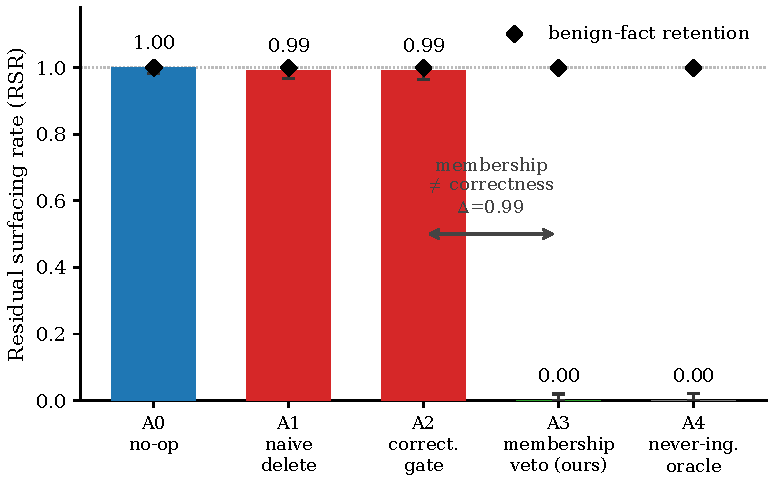
\includegraphics[width=0.48\linewidth]{figures/retract_ladder.pdf}
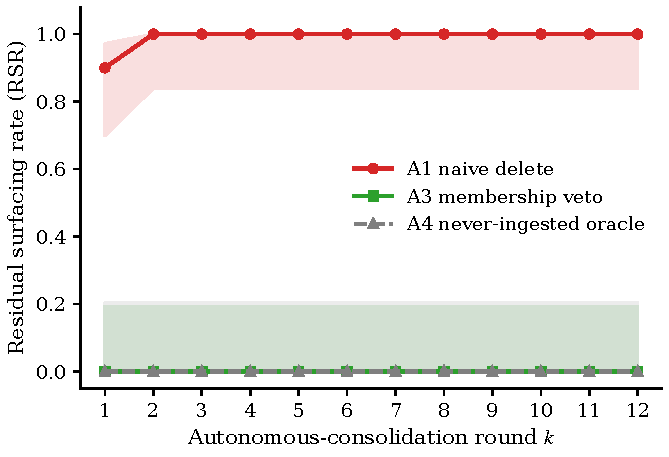
\includegraphics[width=0.48\linewidth]{figures/retract_ksweep.pdf}
\caption{Left: residual surfacing rate across the A0 (no-op)--A4 (never-ingested oracle) arm ladder. Right: surfacing rate across 12 rounds of native consolidation --- the correctness-gated arm rises back toward the no-deletion baseline within two rounds; the membership-gated arm stays flat at zero.}
\label{fig:retract-ladder}
\end{figure}

\paragraph{Scope.} We replicate the effect under the agent's own native (auto-triggered) consolidation loop, not only a scripted harness, and probe a second, architecturally distinct memory substrate (a block-plus-archival agent architecture). We state the scope of that second-substrate result precisely rather than as a second full replication: it is a directional probe ($n{=}24$) with a noisy no-op control ($A0{=}0.88$ rather than the expected $\approx\!1.0$), and it tests the architecture's memory blocks rather than its full agentic tool-call loop. We describe the overall evidence as \emph{two substrates plus a directional second-model probe}, not two independent paradigms or two model families confirming each other --- the $n{=}24$ evidence supports this narrower framing and no stronger one.

\subsection{A complementary result: refusing leakage at serving time}

We additionally target a related but distinct problem: even with a sound deletion gate at the write path, a backbone model may still leak a retracted fact from its own parametric memory when asked directly, independent of what the compiled store contains. We build a serving-time refusal gate for compiled wikis and measure it against a RAG-drop baseline (removing the source's chunk from the retrieval index, but not gating the model's own recall): on correct-and-retracted queries, the gated system leaks $0\%$ of the time against $100\%$ for the RAG-drop baseline. This is an architectural result --- the gate refuses by construction, the RAG-drop baseline surfaces by construction --- and is independent of any statistical estimator. We report it with its own honest caveats: the correct-and-retracted stratum is small ($n{=}15$), giving a wide confidence interval, and the backbone and the judge share the same underlying model family, a circularity risk we flag explicitly.

We also explored a formal criterion for a harder case: a claim in the compiled wiki whose content is \emph{fused} from two or more sources, so that retracting one source cannot be done by deleting a single sentence. We do not carry that formal criterion into this paper. Our own analysis found the proposed residue metric structurally blind to exactly the fused-claim case it was built to detect: by the metric's own definition, a fused claim already has no single source that entails it above threshold, which is also the condition the residue check uses to declare success --- so the metric cannot distinguish a claim that correctly dropped the retracted source's contribution from one that never could have revealed it. We do not use it. \textbf{Formally certifying removal of one source's marginal contribution to a claim that several sources jointly support remains an open problem}, and we name it as such rather than presenting a partial or contested solution as settled.
